\section{VDMS Design \& Implementation}
\label{arch}

In this section, we further describe VDMS design principles and implementation,
which was briefly introduced in previous work \cite{vdms-nips}.
VDMS implementation is fully open-sourced
\footnote{https://github.com/IntelLabs/vdms}.

\begin{figure}
\centering
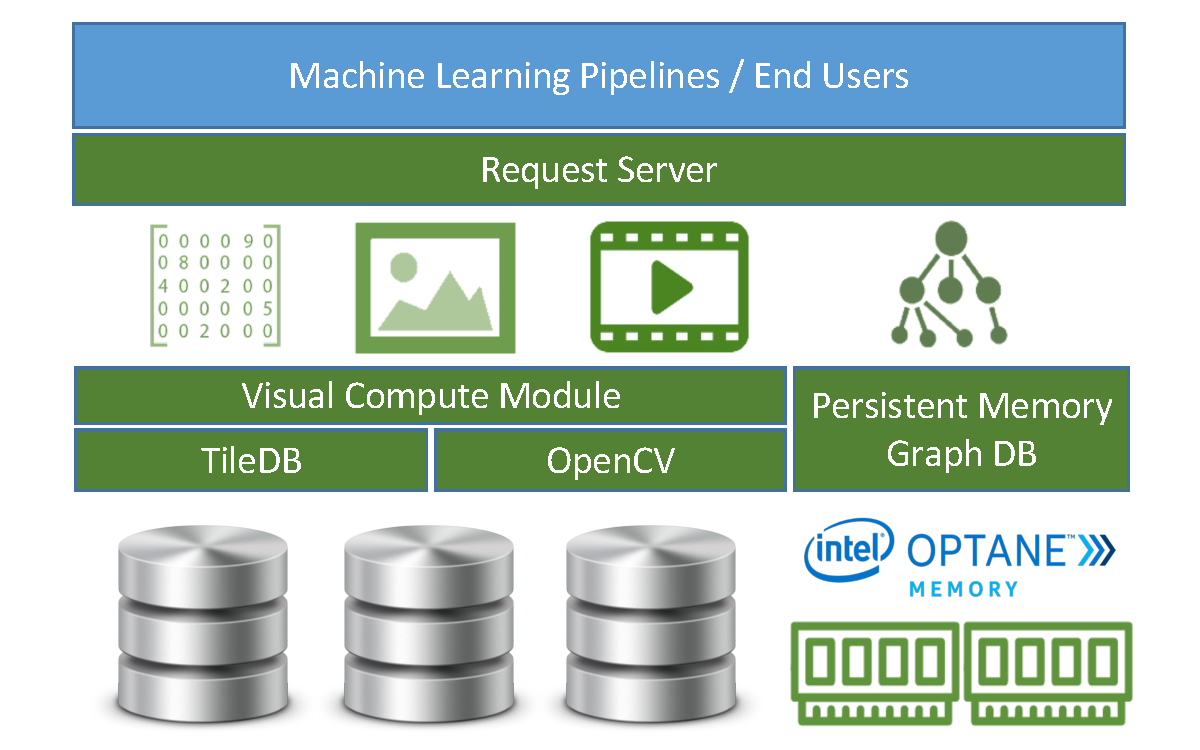
\includegraphics[width=1\columnwidth]{figures/vdms_arch.pdf}
\caption{VDMS Architecture}
\label{fig:arch}
\end{figure}

VDMS implements the typical client-server architecture that handles
client queries transactionally and concurrently, similar to what most common
relational and non-relational database systems
\cite{mysql, postgresql, chang2008bigtable} use.
The main difference between other data management systems and VDMS is that
it goes beyond the typical supported data types (string, integers, floats,
blobs, JSON-documents, etc), recognizing visual entities (image, videos,
feature vectors, etc) as first class citizens.
VDMS API enable users to insert, index, process, and query visual data,
as well as provides full support for inserting, indexing and querying
user-defined metadata.
Users interact with both metadata and visual data using a unified API,
in a transactional manner.

VDMS provides a \textit{graph model} abstraction with the traditional
atomicity, consistency, isolation, and durability
(ACID) properties expected from databases.
This is, users interact with their objects (metadata, images, videos, etc),
as if these objects were in a connected graph.
Graph represents an easier abstraction to model complex problems,
making it very suitable for the data and access patterns shown by visual metadata,
which can be easily mapped into application-level abstractions by
developers~\cite{tao}.
For instance, abstractions like \textit{BoundingBoxes} associated to
images or videos can be easily represented using nodes and edges in a graph.
This is the main reason why the team chose a graph model over a
relational one for the implementation of VDMS API.

VDMS API provides a mechanism to insert and connect Images, Videos, BoundingBoxes,
Frames, and Descriptors (feature vectors), together with any metadata
associated with the objects.
Each object is a node in the graph.
The information associated to each visual object (image, video, etc) is modeled as
"properties" of the node in the graph.
Users can query, filter, and retrieve these objects based on its properties.
VDMS does not simply treat these objects as binary blobs of data, but rather
understands them and the type of processing that is common for them,
providing the ability to run processing on-the-fly, both at insertion and
retrieval time.
Users can, for instance, retrieve a resized version of an image,
or retrieve only a clip from a large video.
This is one of the main differentiating aspects when compared to other
database systems, including relational databases.
In a relational database, for instance, one can query \textit{and compute}
over values in a column only for basic data types (strings, integers, floats),
and over the abstractions the relational model supports (tables, columns).
This is, a SQL query can retrieve the \textit{computed average} "salary" of all
the employees in a company (stored using the table/columns abstraction),
but cannot perform any computation over data stored as a blob or binary object.
VDMS, because it recognized the nature of visual objects by design,
provides the ability to \textit{compute} on these visual objects
(image, videos, etc).

VDMS API also allows users to insert application-defined "Entities",
that enable applications to model any use-case specific metadata.
An "Entity" object (and its properties) is a node in the graph.
For example, a user can define an Entity object of a class "Person",
and \textit{connect} this person to one or multiple image objects.
Later, the user can retrieve the Entity object corresponding to a person,
together with all the images \textit{connected} to it.

By providing the ability to store visual data objects together with
application-defined entities and its properties, VDMS can manage
all the data the application need behind a single, unified API.
This is in contrast with current applications that rely on a combination
of multiple data management systems and APIs to access different
portions of the data they need
\cite{tao, sculley2015hidden, mayer2020scalable, sculley2015hidden}.

Figure \ref{fig:arch} depicts the high-level architecture of VDMS, which
is composed by several subcomponents, and a Query Engine that implements
the unified API and hides all the complexity underneath.
We first describe the VDMS API, and then describe its subcomponents
and design decisions.

\subsection{VDMS API}

One of the most important differentiating aspects of VDMS is its API.
VDMS is unique in recognizing visual entities (i.e., images, videos, etc)
as first class citizens.
Thus, VDMS' API revolves around visual data operations and retrieval,
but at the same time, enables applications to store any other
application-specific metadata.
VDMS API is easy to use and explicitly pre-defines certain
primitives associated with metadata, images, videos, and feature vectors.
Authors have paid particular attention to hide the complexities of our internal
implementation and up-level the API to a JSON-based API,
which is very popular across various application domains.
By defining a new JSON-based API, there is a trade-off between expressiveness
(compared to well-established query languages like SPARQL, Gremlim, or even SQL)
and the ability to natively support visual data operations.
However, we believe it is possible for our API to achieve similar levels of
expressiveness compared to more mature query languages over time.

Listing~\ref{addimageandautotag} shows a sample query for inserting
an image, properties associated with the image, and metadata to VDMS.
The metadata, in this case, is the information about the "autotag",
which is provided by the dataset in this specific
\textit{image-search} application.
In this example, the transaction inserts an application-defined "Entity" of
the class "autotag", with the "name" property being \textit{alligator},
inserts an Image with its "latitude" and "longitude",
stores the image as a JPG (VDMS will transcode if needed),
and creates a connection between the Image and the Entity, with a "prob"
property (which indicates the probability of that image
containing an object of type  \textit{alligator}) with a specific value.
This query is performed \textit{transactionally}: either all the image, metadata
and connection are inserted, or none of them are and an error is returned.
Note that no schema needs to be defined in advance.
The Entity of class "autotag", with its properties, are declared and added
at insertion time, without any need to define a schema of objects
(and its properties) before hand.

\begin{listing}[ht!]
\begin{minted}[frame=single,
              framesep=3mm,
              linenos=true,
              xleftmargin=21pt,
              tabsize=4]{js}
"AddEntity"{
    "_ref" : 1,
    "class": "autotag",
    "properties": {
        "name": "alligator"
    }
},
"AddImage":{
    "_ref": 2,
    "properties": {
        "latitude":  36.23433,
        "longitude": -116.80666
    },
    "format": "jpg"
}
"AddConnection": {
    "ref1": 1,
    "ref2": 2,
    "properties": {
        "prob": 0.7653
    }
}

\end{minted}
\caption{Sample Query for Image Insertion -
The query expresses the following:
Insert an Entity of the class "autotag", with the "name" property being
\textit{alligator}, insert an Image with its "latitude" and "longitude",
store the image  as a JPG, and create a connection between
the image and the "autotag",  with a property "prob"
(which indicates the probability of that image
containing an object of type  \textit{alligator}).}
\label{addimageandautotag}
\end{listing}

Listing~\ref{findimagegeo} shows another sample query, in this case, for retrieval.
In this particular example, the transaction retrieves all the images
of \textit{alligators} with probability higher than 0.66,
filter by latitude and longitude within 1 degree,
apply a resize operation to make the images 224x224,
rotate the images 45.34 degrees, and return the images as "png" files.
It is important to note how the API natively supports basic building
blocks of visual data processing, like resize, rotation, or transcoding
(changing output formats and encodings).
The API allows interaction with metadata, images, videos, bounding boxes,
frames, feature vectors, and more in a similar fashion,
and it is fully documented on the project's Github
wiki~\footnote{https://github.com/IntelLabs/vdms/wiki/API-Description}.

\begin{listing}[ht!]
\begin{minted}[frame=single,
              framesep=3mm,
              linenos=true,
              xleftmargin=21pt,
              tabsize=4]{js}
"FindEntity"{
    "class": "autotag",
    "constraints": {
        "name": ["==", "alligator"]
    }
    "_ref" : 1
},
"FindImage":{
    "format": "png",
    "constraints": {
        "latitude": [">=", 36.23433,
                     "<=", 38.23433]
        "longitude":[">=", -114.80666,
                     "<=", -116.80666]
    },
    "operations": [{
            "type": "resize",
            "height": 224,
            "width":  224,
        }, {
            "type": "rotate",
            "angle": 45.34
    }],
    "link": {
        "ref":1,
        "constraints": {
            "prob": [">=", 0.66]
        }
    }
}

\end{minted}
\caption{Sample Query for Image Retrieval -
The query expresses the following:
Find all the images connected to the autotag \textit{alligator}
with probability higher than 0.66,
filter the images by latitude and longitude within 1 degree,
apply a resize operation to make the images 224x224,
rotate the image 45.34 degrees,
and return the images as "png" files.}
\label{findimagegeo}
\end{listing}

\subsection{Graph Engine}

The Graph Engine used in VDMS is the
\textit{Persistent Memory Graph Database} (PMGD).
PMGD was developed at Intel Labs, and was designed and optimized for
persistent memory technologies like Intel Optane~\cite{IntelXPoint15}, which
promise storage providing nearly the speed of DRAM and the
durability of block-oriented storage.
PMGD is also fully open-sourced \footnote{https://github.com/IntelLabs/pmgd}.
PMGD implements an in-persistent-memory graph database optimized
to run on a platform equipped with persistent memory, but
also provides the option to run on SSD and ext4 filesystem
using OS support to provide transactional guarantees (through \textit{msync}).
PMGD provides a property graph model of data storage with the traditional
atomicity, consistency, isolation, and durability
(ACID) properties expected from databases.
PMGD comes as a C++ library that VDMS uses for implementing its query engine.
Because PMGD already supports most of the graph abstractions we wanted
to see on VDMS API, it was our preferred option.
Also, our internal evaluation shows that PMGD is faster
than other graph databases, including Neo4j\cite{miller2013graph}.
PMGD performance evaluation will be published separately.

\subsection{Visual Compute Module}

% The Visual Compute Module enables machine-friendly enhancements to
% visual data, exposing high-level abstractions to the \textit{Request Server}
% for dealing with a variety of images and video formats (through OpenCV and ffmpeg),
% and different methods for indexing for feature vectors
% (including Facebook's Faiss \cite{faiss}, TileDB \cite{TileDB}).
% Finally, a main component of VDMS is in charge of implementing the
% API and orchestrating between the PMGD and the Visual Compute Module
% to serve client's requests. This component is the \textit{Request Server}.

The Visual Compute Module was designed and implemented to provide
an internal abstraction layer for interacting with visual data.
It enables the query engines to coordinate and perform
visual data handling and processing
(i.e., basic building block operations like crop, resize, etc for images/videos
and k-nearest neighbor search for feature vectors),
shown in Figure \ref{fig:arch}.
For traditional formats (jpg, png, tiff, mp4, etc.),
the interface is an abstraction layer over OpenCV.
However, it also provides a way to use novel formats that are
better suited for visual analytics: a novel, array-based lossless image format.
This format is built on the array data manager TileDB~\cite{TileDB} and
is well suited for images that are used in visual analytics.
Note that, even if VDMS currently provides support for array-based lossless
image format, we do not use it as part of this evaluation.
This work focuses on a more direct comparison with a combination of alternatives,
and thus we use the traditional format (jpg and png).
The performance comparison between the array-based lossless image format
we develop and other similar formats (like png or tiff) are outside of the
scope of this evaluation.

VDMS also provides full support for video storage and operations,
in a similar way it does for images.
This includes support for encoding, decoding, and transcoding of
\textit{mp4}, \textit{avi}, and \textit{mov} containers,
as well as support for \textit{xvid}, \textit{H.263} and \textit{H.264} encoders.
This is supported through the use of either OpenCV~\cite{opencv}
or \textit{libffmpeg}\cite{ffmpeg}, or both,
plus additional implementation to support fast random access to video frames.
All operations supported for images in VDMS are also supported at the
video and frame level of the API.
On top of that, there are a number of video-specific operations that
are supported, such as the interval operations,
enabling users to retrieve clips at different
frames-per-second (fps) versions of the video.

Another key differentiating factor of VDMS is that it allows the creation of
indexes for high-dimensional feature vectors and the insertion of
these feature vectors associated with entities, images, and/or videos.
Feature vectors are intermediate results of various machine
learning or computer vision algorithms when run on visual data.
Feature vectors are also known as \textit{descriptors}
or \textit{visual descriptors}.
We use these terms interchangeably.
These descriptors can be classified, labeled, and used to build search indexes.
Feature Vectors support is provided through our implementation based
on high-dimensional sparse arrays, also using array-based approaches.
In addition, the Visual Compute Library provides a wrapper
for another high-dimensional index implementation,
Facebook's Faiss~\cite{faiss}.
Users can, through our API, use different indexing techniques
for feature vectors, depending on their application's need.


\subsection{Client Library}

The client library implements TCP/IP based connectors to the VDMS Server,
similar to most databases\cite{memsql, mysql, postgresql}.
Users can connect to VDMS and run queries using VDMS' API
by defining a transaction using JSON objects.
The client library provides a simple method that
accepts a JSON string and an array or vector of blobs.
Internally, the library wraps the query string and blobs using
Google Protobufs \cite{protobufs} and sends it to the VDMS server.
It also receives a similarly formed response from VDMS
and returns it to the client.
Currently, client libraries are implemented for Python and C++ client.
The client libraries are lightweight, as they simply implement the communication
protocol between the client and the server.
This makes it easier for developers to implement similar client libraries using
any other programming language of their choice.
